\pdfminorversion=4
\documentclass[aspectratio=169]{beamer}
\usepackage{verbatim}
\newenvironment{metaverbatim}{\verbatim}{\endverbatim}
\usepackage{courier}
\usepackage{lmodern}
\usepackage{apacite}
\usepackage[hidelinks]{hyperref}
\usepackage{xcolor}
\xdefinecolor{azulcesafuerte}{HTML}{14387e}
\xdefinecolor{azulcesaclaro}{HTML}{7ab6e0}
\xdefinecolor{azulcesamedio}{HTML}{0A72BC}

\usetheme{Madrid}
%\usecolortheme[named=black]{structure}
%
\setbeamercolor{normal text}{fg=azulcesafuerte}
\setbeamercolor{background canvas}{bg=white}
\setbeamercolor{frametitle}{fg=white, bg=azulcesafuerte}
\setbeamercolor{block title}{bg=azulcesafuerte,fg=azulcesaclaro}
\setbeamercolor{navigation symbols}{}

\setbeamertemplate{background}{\tikz[overlay,remember picture]\node[opacity=0.15]at (current page.center){\includegraphics[width=6.5cm]{}};}
\usepackage{tikz}
\usepackage{kantlipsum}
\setbeamercolor*{title}{fg=white, bg=azulcesafuerte}
\setbeamercolor{titlelike}{parent=structure}

\setbeamercolor*{palette primary}{bg=azulcesafuerte,fg=white}
\setbeamercolor*{palette secondary}{bg=azulcesafuerte,fg=white}
\setbeamercolor*{palette tertiary}{bg=azulcesafuerte,fg=white}

% Change base colour beamer@blendedblue (originally RGB: 0.2,0.2,0.7)
\colorlet{beamer@blendedblue}{azulcesaclaro}
\usepackage[english]{babel}
\usepackage{apacite}
\usepackage{marvosym}
\usepackage{subfig}
\usepackage{graphicx}
\usepackage[utf8x]{inputenc}
\usepackage{url}
\usepackage{hyperref}
\usepackage{times}
\usepackage{pxfonts}
\usepackage{fontenc}
%\usepackage[dvipsnames]{xcolor}
\setbeamertemplate{bibliography item}[text]
\title[Fuentes de Datos: Relevancia para Los Negocios]{Fuentes de Datos: Relevancia para Los Negocios}
\subtitle{(Sesión 3B)}

\author[Prof. Juan C. Correa, Ph.D.]{Prof. Juan C. Correa, Ph.D.}

\institute[]{
Colegio de Estudios Superiores de Administración\\
Bogotá - Colombia\\
% \color{azulcesaclaro}\Email  \href{mailto:juan.correan@cesa.edu.co}{juan.correan@cesa.edu.co}
}
\pgfdeclareimage[height=0.6cm]{OL}{OL}
 \logo{\pgfuseimage{OL}}
 \setbeamertemplate{caption}[numbered]
\date[Bogotá, Agosto, 2021] % (optional)
{}

\subject{}
\begin{document}
\begin{frame}
\titlepage
\end{frame}

% \begin{frame}
% \frametitle{Agenda} 
% \tableofcontents
% \end{frame}

\begin{frame}
\begin{block}{Objetivo de Aprendizaje}
Normalmente, los gerentes toman decisiones considerando los datos sobre algunos aspectos de las operaciones comerciales de sus negocios (e.g., ventas, cobranzas, producción). En la práctica, sin embargo, estos datos tienen características indeseables que impiden su uso inmediato (e.g., datos desordenados, incompletos, o con errores). Al finalizar esta sesión de clases, usted estará en capacidad de comprender la relevancia de las fuentes de datos como insumos para la comprensión de realidades estudiadas desde la perspectiva de la analítica de datos.
\end{block}
\end{frame}


\section{Conceptos Preliminares}
\begin{frame}
\begin{center}
\Huge
\textcolor{azulcesaclaro}{1\\
--------------------------------\\
Conceptos Preliminares:\\
Datos, Información, Conocimiento, Sabiduría}
\end{center}
\end{frame}

\begin{frame}
En la presentación del curso (slides 8-9) se introdujo el concepto de \textbf{Jerarquía de la Sabiduría} \cite{Rowley2007}. Para comprender este concepto, se debe asimilar la diferencia conceptual que existe entre datos, información, conocimiento y sabiduría. \citeauthor{Zins2007} \citeyear{Zins2007} definió esta diferencia así:\\
\vspace{0.3cm}
\begin{itemize}
\item \textbf{Datos} (viene del latín \textit{datum}: ``lo que ocurrió, lo que se da''). Un registro alfanumérico que representa una observación.
\item \textbf{Información}: La síntesis o el resumen de un conjunto de datos.
\item \textbf{Conocimiento}: El otorgamiento de significado práctico que conlleva la información.
\item \textbf{Sabiduría}: Principios o valores de juicio que orientan nuestro proceder ético y moral. 
\end{itemize}
\end{frame}

\begin{frame}
La distinción planteada por \citeauthor{Zins2007} \citeyear{Zins2007} se apoya en la diferenciación entre el reino de lo objetivo y lo subjetivo.  El reino de lo objetivo implica todo aquello cuya existencia es externa a la conciencia de cada persona (e.g., las longitudes de onda de la luz reflejadas sobre un cuerpo). El reino de lo subjetivo implica todo aquello cuya existencia está en la conciencia de cada individuo (e.g., la sensación de color azul oscuro versus azul claro).
\begin{figure}
\centering
 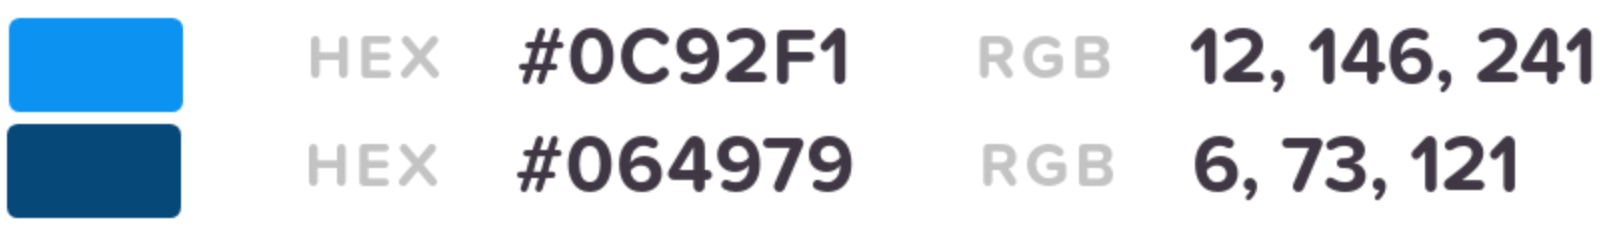
\includegraphics[width=.8\textwidth]{colores.png}
\end{figure}
\end{frame}


\section{Fuentes de Datos}
\begin{frame}
\begin{center}
\Huge
\textcolor{azulcesaclaro}{2\\
--------------------------------\\
Fuentes de Datos\\
¿Qué son? ¿dónde están?\\
¿Para qué sirven?}
\end{center}
\end{frame}

\begin{frame}
Taller Guiado:\\
En parejas, un estudiante debe explorar las siguientes fuentes de datos:
\begin{itemize}
    \item \url{https://rda.ucar.edu/}
    \item \url{https://datadryad.org/stash}
    \item \url{http://archive.eso.org/cms.html}
    \item \url{https://www.dataone.org/}
    \item \url{https://figshare.com/}
\end{itemize}
Otro estudiante debe explorar las siguientes fuentes de datos.
\begin{itemize}
    \item \url{https://www.icpsr.umich.edu/web/pages/}
    \item \url{https://www.re3data.org/}
    \item \url{https://ciser.cornell.edu/data/data-archive/}
    \item \url{https://dataverse.harvard.edu/}
    \item \url{https://www.europeansocialsurvey.org/}
\end{itemize}
\end{frame}


\begin{frame}
Taller Guiado (continuación slide previo):\\
Para explorar cada fuente de datos, usted debe:\\
\begin{itemize}
\item Buscar la sección ``\textbf{About}'', leer la descripción allí escrita y tomar nota de esa información.
\item Observar los temas asociados con cada base de datos y seleccionar un tema en específico que sea de su interés (e.g., Covid, Deportes, Bitcoin, etc.)
\item Descargar la base de datos que más llame su atención. 
\item Intentar abrir la base de datos y documentar (en un documento de Word) qué datos contiene dicha base de datos, por qué la seleccionó, incluir su dirección URL y describir brevemente cómo podría extraer información valiosa para la generación de conocimiento útil a partir de dicha base de datos. 
\end{itemize}
\end{frame}

\section{Extracción de información a partir de datos}

\begin{frame}
\begin{center}
\Huge
\textcolor{azulcesaclaro}{3\\
--------------------------------\\
Extracción de información\\
a partir de datos}
\end{center}
\end{frame}

\begin{frame}
En un mundo ideal, las bases de datos ya están listas para ser usadas inmediatamente con propósitos de extracción de información. \\
\vspace{0.3cm}
En el mundo real, las bases de datos son hechas por personas sin formación en estadística, o personas que simplemente ignoran los principios básicos que se enseñan en las primeras clases de analítica de datos. Aquí aprenderemos estos principios básicos.
\end{frame}

\subsection{Manipulación de datos}
\begin{frame}
\begin{center}
\Huge
\textcolor{azulcesaclaro}{3.1\\
--------------------------------\\
Manipulación de datos\\
(Data Wrangling)}
\end{center}
\end{frame}

\begin{frame}
La manipulación de datos (data wrangling) agrupa al conjunto de procedimientos dirigidos a resolver las deficiencias que presentan las bases de datos tal y como fueron elaboradas desde su origen \cite{Shmueli2020}. Algunas deficiencias típicas son:
\begin{itemize}
\item Bases de datos desordenadas
\item Bases de datos sin las variables relevantes
\item Bases de datos con casos perdidos
\item Bases de datos con observaciones incompletas
\item Bases de datos con errores de transcripción o escritura
\item Bases de datos en formatos ineficientes (¡Sí, Excel es un formato ineficiente!)
\item Bases de datos con registros repetidos, duplicados o falsos.
\item Multiplicidad de bases de datos, cada una con su propio formato y sus propias deficiencias.
\end{itemize}
\end{frame}

\begin{frame}
¿Cuál es la estructura de una \textbf{base de datos ordenada}?\\
\vspace{0.5cm}
Una base de datos es ordenada cuando, cada variable ocupa una columna, cada observación  ocupa una fila, y cada dato ocupa una celda.
\begin{figure}
\centering
 
\includegraphics[width=.8\textwidth]{tidy.png}
\end{figure}
Cualquier desviación de estas reglas implica automáticamente una base de datos desordenada.
\end{frame}

\subsection{Manipulación de datos}
\begin{frame}
\begin{center}
\Huge
\textcolor{azulcesaclaro}{3.2\\
--------------------------------\\
Práctica Guiada con Python Pandas\\
(Data Wrangling)}
\end{center}
\end{frame}

\begin{frame}
Para practicar con Python Pandas, necesitamos descargar e instalar \href{https://www.anaconda.com/products/individual}{\textcolor{blue}{Anaconda-Navigator}}
\centering
\begin{figure}
\centering
 
\includegraphics[width=.65\textwidth]{Install.png}
\end{figure}
\textcolor{blue}{\url{https://youtu.be/OmmklYlRGzo}}
\end{frame}

\begin{frame}
También necesitamos descargar e instalar \href{https://desktop.github.com/}{\textcolor{blue}{GitHub Desktop}}
\centering
\begin{figure}
\centering
 
\includegraphics[width=.65\textwidth]{GitHubInstall.png}
\end{figure}
\textcolor{blue}{\url{https://youtu.be/tn6tloweTUs}}
\end{frame}


\begin{frame}
Una vez descargado e instalado \href{https://desktop.github.com/}{\textcolor{blue}{GitHub Desktop}}, debemos clonar el siguiente \href{https://github.com/stefmolin/Hands-On-Data-Analysis-with-Pandas-2nd-edition}{\textcolor{blue}{repositorio}}
\centering
\begin{figure}
\centering
 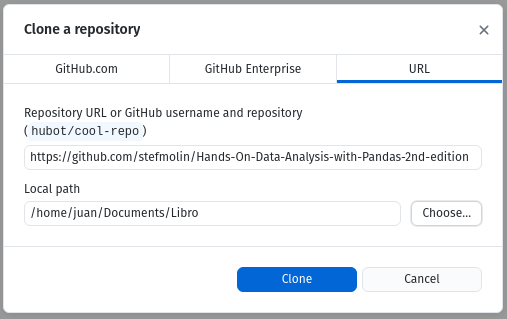
\includegraphics[width=.65\textwidth]{Clonar.png}
\end{figure}
\scriptsize
\textcolor{blue}{\url{https://github.com/stefmolin/Hands-On-Data-Analysis-with-Pandas-2nd-edition}}
\end{frame}

\begin{frame}
Una vez clonado ese repositorio, usted debe ir al explorador de archivo y verificar la existencia de una carpeta llamada \textit{Hands-On-Data-Analysis-with-Pandas-2nd-edition}
\begin{figure}
\centering
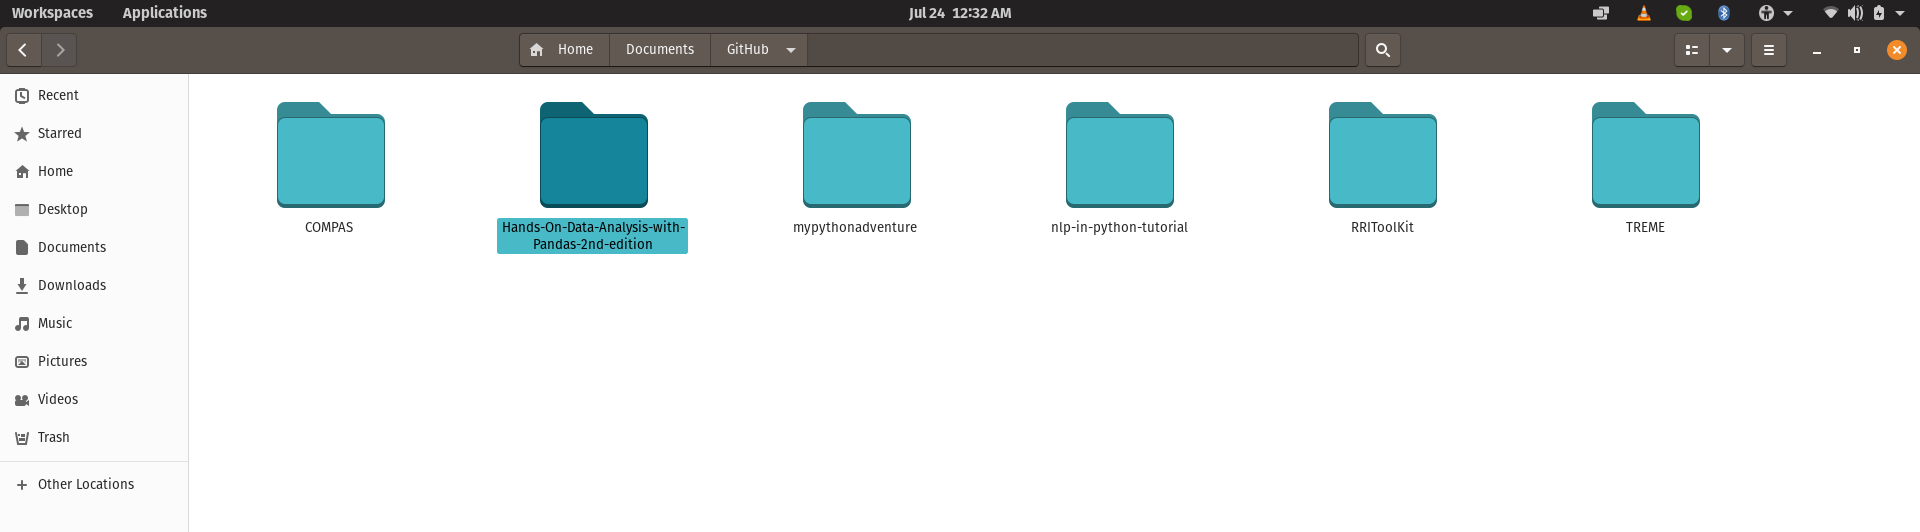
\includegraphics[width=.75\textwidth]{carpeta.png}
\end{figure}
Dentro de esa carpeta, deben haber exactamente 16 subcarpetas (12 carpetas de los 12 capítulos del libro de \citeauthor{Molin2021} \citeyear{Molin2021}, tres subcarpetas adicionales y cuatro archivos.
\end{frame}

\begin{frame}
Hecho lo anterior, ingresamos a anaconda-navigator y hacemos clic sobre el botón de Launch que está justo debajo del ícono de jupyter Notebook
\begin{figure}
\centering
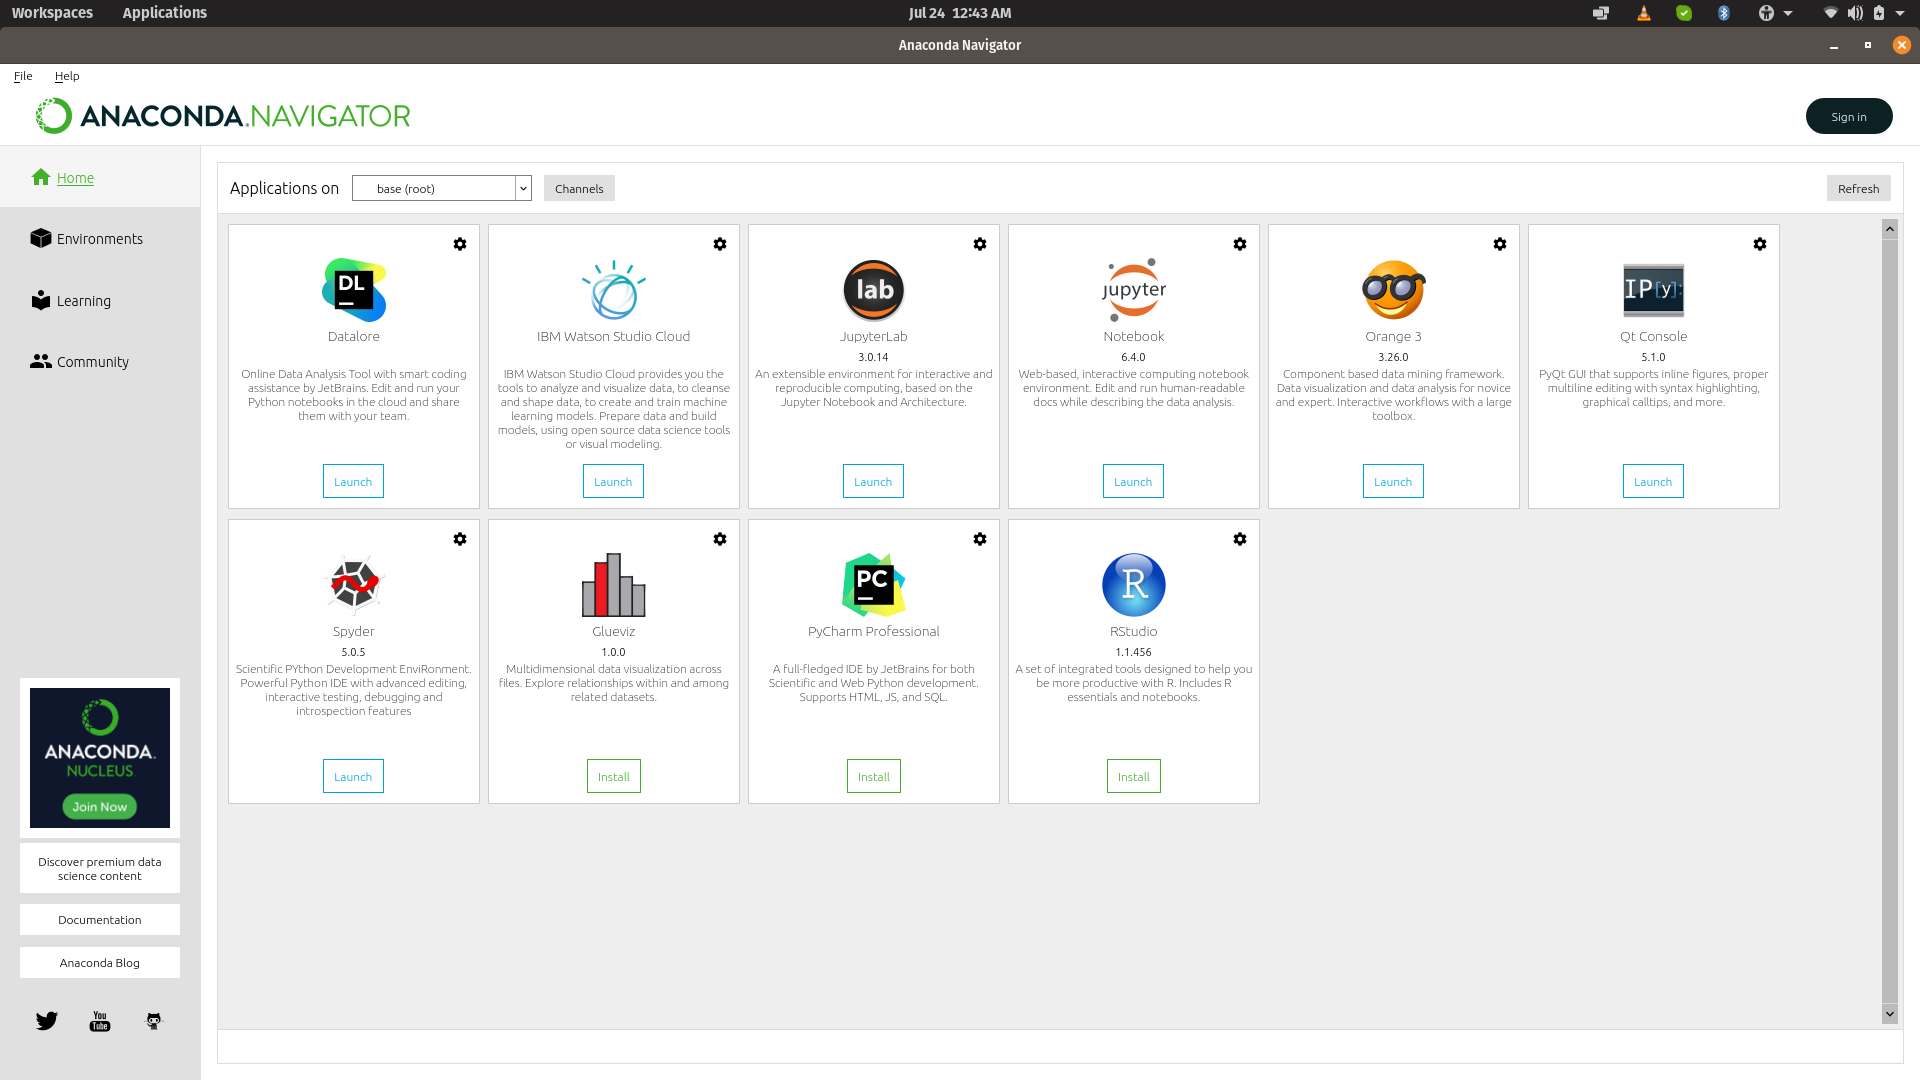
\includegraphics[width=.75\textwidth]{anac.png}
\end{figure}
\end{frame}

\begin{frame}
El resultado visible del paso anterior es que en nuestro navegador de internet predeterminado se abre una nueva pestaña con una página web que muestra el listado de carpetas que tenemos dentro del disco duro de nuestra computadora. Allí debemos buscar la carpeta con el nombre del libro que clonamos de GitHub, buscar la carpeta ch\_03
\begin{figure}
\centering
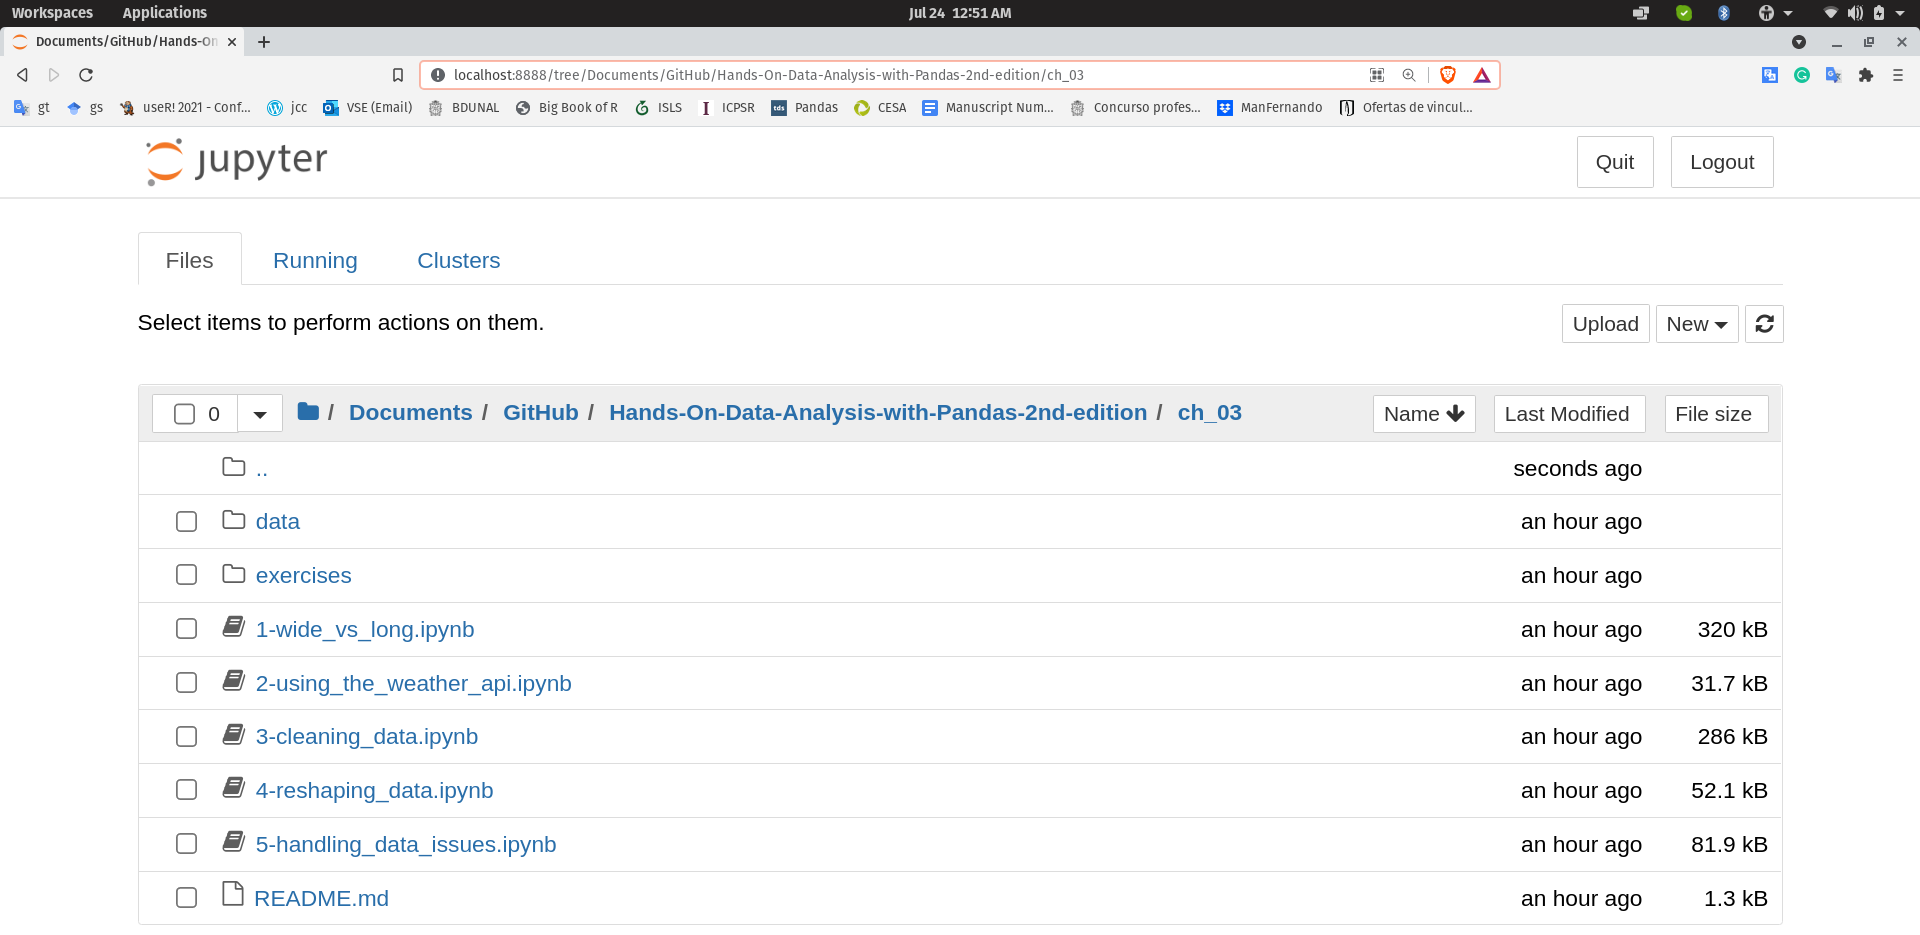
\includegraphics[width=.65\textwidth]{ch_03.png}
\end{figure}
\end{frame}

\begin{frame}
Dentro de la carpeta ch\_03, hacemos clic sobre el archivo \textit{3-cleaning\_data.ipynb}
\begin{figure}
\centering
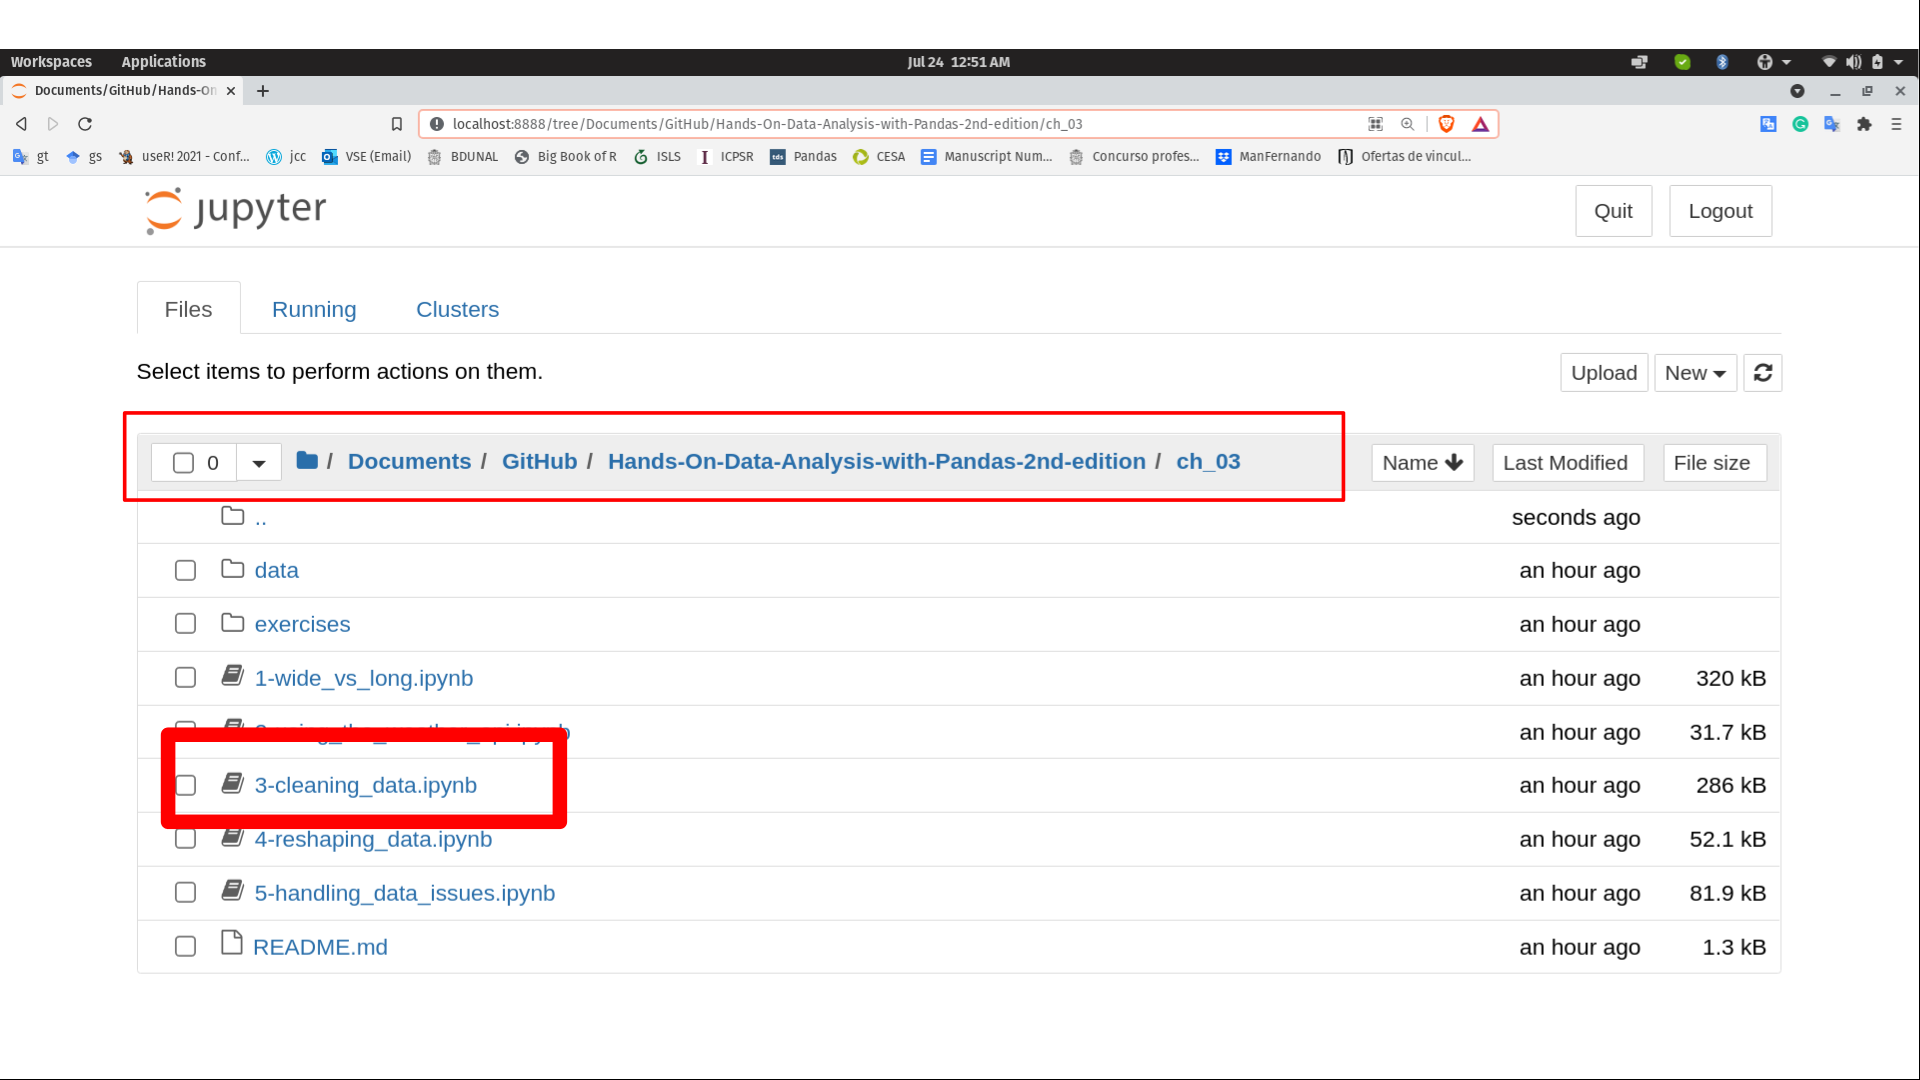
\includegraphics[width=.65\textwidth]{danac.png}
\end{figure}
\end{frame}

\begin{frame}
De haber seguido fielmente la secuencia de pasos descrita hasta este punto, observaremos nuestro primer jupyter Notebook, tal como se observa aquí.
\begin{figure}
\centering
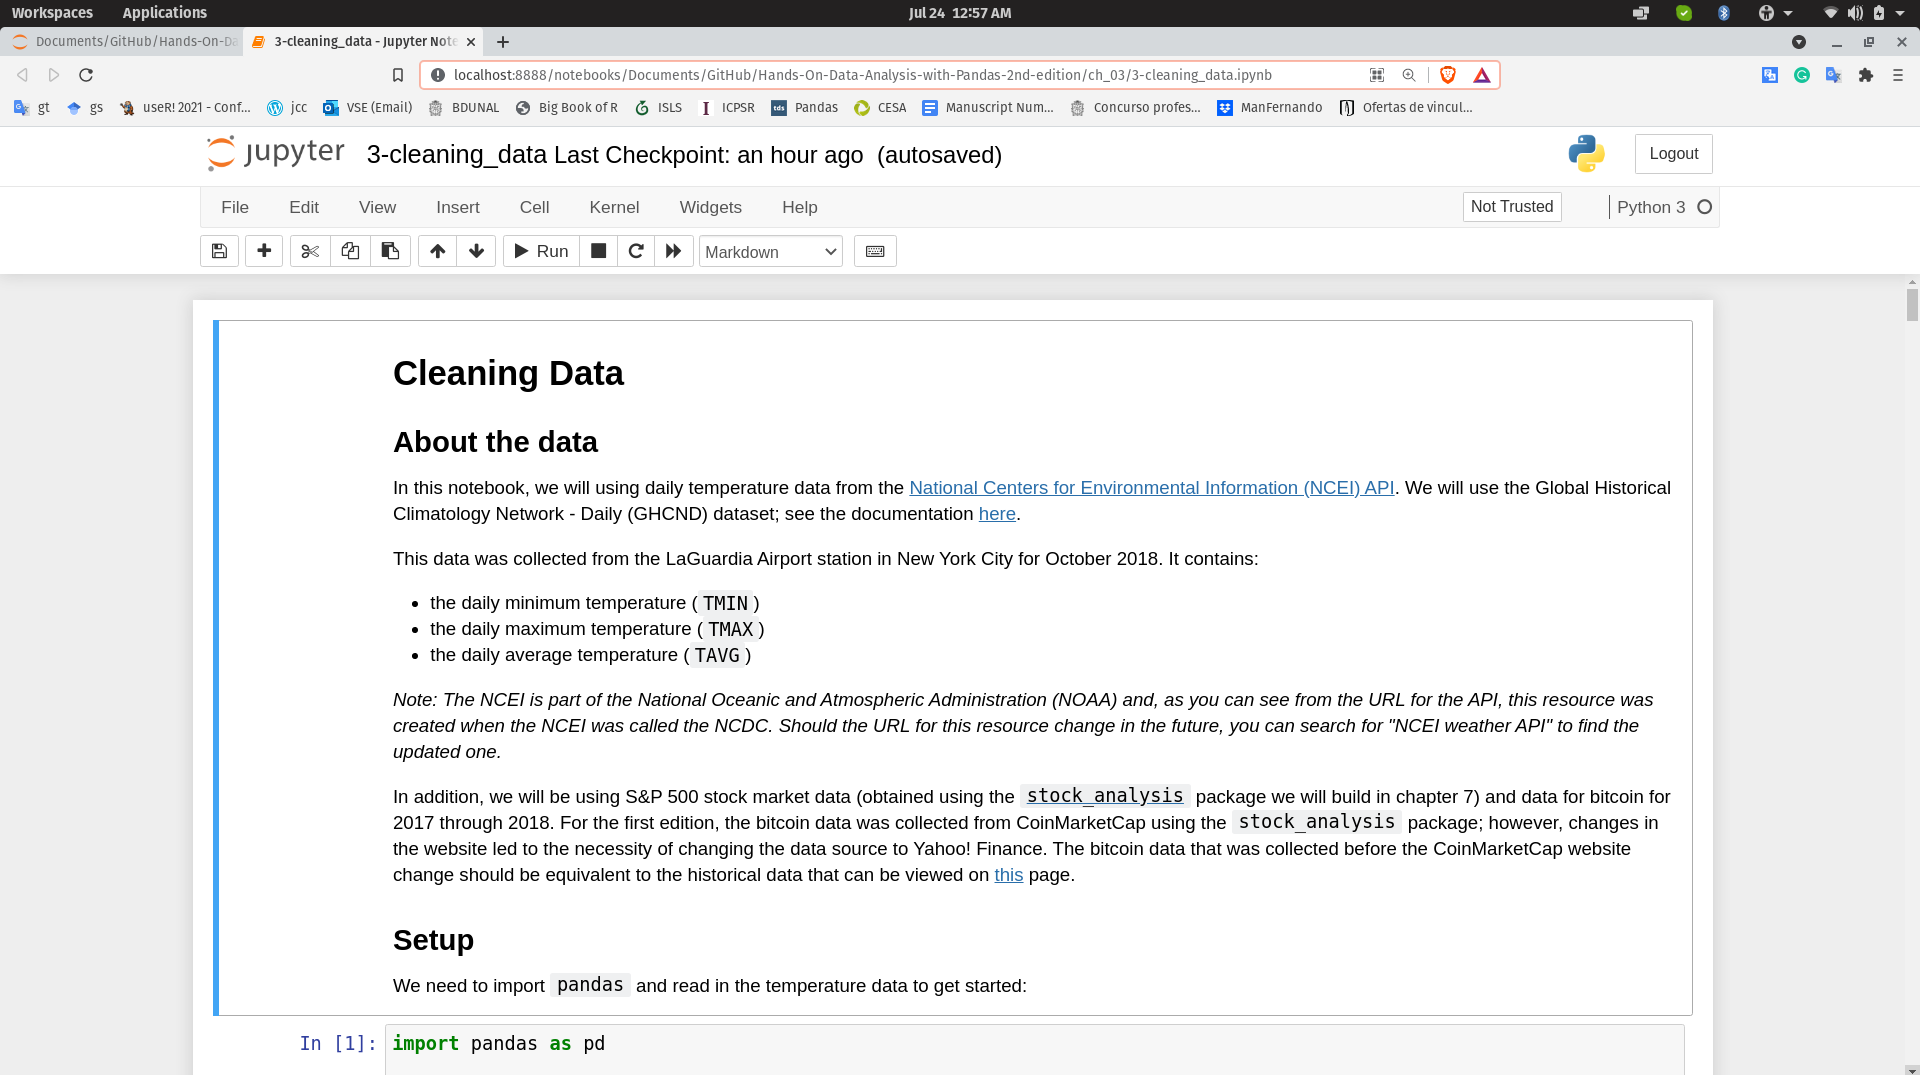
\includegraphics[width=.65\textwidth]{jupyter.png}
\end{figure}
\end{frame}

\begin{frame}
Este jupyter Notebook contiene un total de 42 sintaxis de código en Python. Para entender lo que se hace con estas sintaxis, basta con leer el texto que antecede a cada código para enteder que estamos haciendo con esta herramienta.\\
\vspace{0.3cm}
\begin{itemize}
\item ¿Cuál es la base de datos que se abre con ese jupyter Notebook?
\item ¿Cuál es la extensión de la base de datos que se está abriendo con este jupyter Notebook?
\item ¿A partir de cuál línea de código se empieza a hacer Reordering, reindexing, and sorting?
\end{itemize}
\end{frame}

\section{Trabajo Independiente}

\begin{frame}
\begin{center}
\Huge
\textcolor{azulcesaclaro}{4\\
--------------------------------\\
Trabajo Independiente}
\end{center}
\end{frame}

\begin{frame}
En el libro de \citeauthor{Molin2021} \citeyear{Molin2021}, los capítulos 4, 5, y 6 abordan otros aspectos de Data Manipulation. Su trabajo independiente consiste en repetir los pasos descritos en esta presentación para estudiar los aspectos de:\\
\vspace{0.3cm}
\begin{itemize}
\item Agregación de dataframes (Capítulo 4)
\item Visualización de datos con Pandas (Capítulo 5)
\item Técnicas de graficación y personalización con Seaborn (Capítulo 6).
\end{itemize}
\end{frame}



\section*{REFERENCIAS}
\begin{frame}[allowframebreaks]{Referencias}
\tiny{ 
\bibliographystyle{apacite}
\bibliography{REFS.bib}
} 
\end{frame}

\setbeamertemplate{background}{\tikz[overlay,remember picture]\node[opacity=1]at (current page.center){
\includegraphics[width=18cm]{ulam.png}};}
\pgfdeclareimage[height=0cm,width=0cm]{}{}
 \logo{\pgfuseimage{}}
\beamertemplatenavigationsymbolsempty
\begin{frame}
\end{frame}


\end{document}